\documentclass[12pt]{article}
\usepackage{natbib}
\usepackage{amsmath}
\usepackage{graphicx}
\usepackage{geometry}
\usepackage{subcaption}
\usepackage{float} 

\usepackage{amsmath}
\usepackage{graphicx}
\usepackage{subcaption} 
\usepackage{siunitx}    
\usepackage{placeins}   
\usepackage{tikz}
\usetikzlibrary{shapes.geometric, arrows}
\usepackage[margin=1in]
{geometry}\geometry{a4paper, margin=1in}
\usepackage{times}


\newcommand\wordcount{%
  \immediate\write18{texcount -sum -1 main.tex > wordcount.txt} % 
  \input{wordcount.txt} % 
}


\title{Systematic Comparison of Six Microbial Growth Models: Evaluation of Convergence, Parameter Estimation, and Predictive Performance}
\author{Yumeng Huang}
\date{\today}

\begin{document}
\maketitle

% 
\noindent \textbf{Word Count:} \wordcount

\begin{abstract}
My study evaluated six microbial growth models using 4,387 observations from ten sources, refined to 210 datasets. The modified Gompertz model showed the best fit based on AICc, BIC, and Akaike weights, followed by the Baranyi model. The Logistic model had the highest convergence failure rate due to its symmetric growth assumption. Polynomial and three-phase linear models were stable but lacked biological interpretability. Overall, the modified Gompertz model provided the best balance between accuracy and biological relevance. Future research should enhance experimental design and data collection for better model performance.
\end{abstract}


\section{Introduction}

Understanding and predicting microbial growth dynamics is crucial, particularly in the field of food safety \citep{BaranyiRoberts1994}. For instance, the risk of foodborne infections is closely related to the number of microorganisms present in food at the time of consumption \citep{RossMcMeekin2003}. Mathematical models serve as essential tools for predicting and controlling the growth, survival, and death phases of bacteria \citep{LoGrasso2023}. Therefore, systematically evaluating the applicability of these models is of great importance.

However, due to the inherent uncertainties in all models, there is no universally recognized optimal model across different datasets \citep{Marks2008}. For example, in food safety research, environmental factors such as temperature, pH, and nutrient composition can significantly influence microbial growth patterns, yet these factors may not be fully accounted for in certain models \citep{RossMcMeekin2003}. Nevertheless, researchers can assess the relative support of each model based on observed data to determine the most suitable one \citep{JohnsonOmland2004}.

The primary objective of this study is to systematically compare the predictive performance of six bacterial growth models by fitting them to growth curves recorded under different experimental conditions, aiming to identify the most appropriate model. Unlike previous studies that have primarily focused on a single model or specific experimental conditions, the novelty of this research lies in its systematic comparison across multiple datasets. By evaluating the applicability of different models under varying data characteristics, this study provides a scientific basis for improving microbial growth predictions.

\section{Methods}

\subsection{Data}
I used the dataset \texttt{LogisticGrowthData.csv}, which contains 4,387 observations from ten different sources. The dataset records changes in biomass over time under varying temperature conditions and culture media for different microorganisms. First, I generated a unique dataset identifier (ID) based on four categorical variables: Species, Temperature, Medium, and Citation, resulting in 285 unique datasets. To ensure data quality, I removed erroneous data where time was less than 0 or biomass was less than or equal to 0. Additionally, datasets with fewer than eight data points per ID were excluded to prevent fitting failures or inaccuracies. After filtering, 210 valid datasets remained. Finally, since the PopBio data exhibited heteroscedasticity, I computed the log-transformed biomass (\texttt{logPopBio}) for subsequent model fitting. This transformation was necessary to ensure the accuracy of the analysis \citep{Schaffner1998}.

\subsection{Computing Tools}
All analyses were conducted using R version 4.2.2. Several R packages were employed for data processing, statistical modeling, and visualization. \texttt{dplyr} was used for data manipulation, including filtering, grouping, and summarization, while \texttt{ggplot2} facilitated data visualization, particularly for plotting fitted models and model comparisons. Nonlinear least squares fitting was performed using \texttt{minpack.lm}, which provided robust optimization via the \texttt{nlsLM} function. The \texttt{tidyr} package assisted in reshaping datasets, and \texttt{segmented} was utilized for piecewise regression modeling. Model selection and evaluation were carried out using \texttt{MuMIn}, which enabled Akaike Information Criterion (AIC) and corrected AIC (AICc) computations, and \texttt{broom}, which extracted model summaries using functions such as \texttt{glance()} and \texttt{tidy()}. Additionally, \texttt{readr} was used for efficient reading and writing of CSV files, ensuring smooth data handling throughout the analysis.
\subsection{Model Specification}


I used six different models to fit the data, each describing population growth with different mathematical formulations. The population size at time \(t\) is denoted as \(N(t)\).

The first two models, the Quadratic Polynomial Model and the Cubic Polynomial Model, describe the growth process using quadratic and cubic terms, respectively. Their mathematical expressions are:
\begin{equation}
N(t) = a + b\,t + c\,t^2 \quad 
\end{equation}
\begin{equation}
N(t) = a + b\,t + c\,t^2 + d\,t^3 \quad 
\end{equation}
where \(a\) represents the initial population size, \(b\) is the linear growth coefficient, \(c\) accounts for the quadratic effect, and \(d\) captures additional curvature in the growth trend.

The third model is the Logistic Model, which follows a sigmoidal growth pattern and is expressed as:
\begin{equation}
N(t) = \frac{K e^{r t} N_0}{K + N_0(e^{r t} - 1)} \quad 
\end{equation}
where \(K\) represents the carrying capacity (the maximum population size the system can sustain), \(r\) is the maximum growth rate, and \(N_0\) is the initial population size.

The fourth model is the Modified Gompertz Model \citep{Zwietering1990}, given by:
\begin{equation}
\log(N_t) = N_0 + (K - N_0) \exp \Biggl\{ -\exp \Biggl[ r \cdot e(1) \frac{(t_{\mathrm{lag}} - t)}{(K - N_0)\log(10)} + 1 \Biggr] \Biggr\} \quad 
\end{equation}
where \(r\) is the maximum growth rate, \(t_{\text{lag}}\) represents the lag phase (describing the delay before the onset of exponential growth), \(K\) is the maximum population density, and \(N_0\) is the initial population density.

The fifth model is the Baranyi Model \citep{BaranyiRoberts1994}, which accounts for microbial adaptation before the exponential phase. It is formulated as:
\begin{equation}
\log(N_t) = N_0 + r\,t + \frac{1}{r} \ln\Bigl(e^{-v\,t} + e^{-h_0} - e^{-v\,t-h_0}\Bigr) - \frac{1}{m} \ln \left( 1 + \frac{e^{m\,r\,t + \frac{1}{r}\ln\Bigl(e^{-v\,t} + e^{-h_0} - e^{-v\,t-h_0}\Bigr)} - 1}{e^{m(K - N_0)}} \right) \quad 
\end{equation}
where \(r\) is the maximum growth rate, \(K\) is the carrying capacity, \(N_0\) is the initial population size, and \(t_{\text{lag}}\) is the lag phase duration. The parameters \(v\) and \(m\) describe the transition into and out of the exponential phase, while \(h_0\) quantifies the initial physiological state of the cells.

The sixth model is the Three-Phase Linear Model \citep{Buchanan1997} which describes population growth as a sequence of three distinct phases: lag, exponential, and stationary. Its mathematical expression is:
\begin{equation}
N(t)=
\begin{cases}
N_0, & t \leq t_{\text{LAG}}, \\[6pt]
N_0 + \dfrac{N_{\max} - N_0}{t_{\text{MAX}} - t_{\text{LAG}}}(t - t_{\text{LAG}}), & t_{\text{LAG}} < t < t_{\text{MAX}}, \\[6pt]
N_{\max}, & t \geq t_{\text{MAX}}.
\end{cases} \quad 
\end{equation}
where \(N_0\) is the initial population size, \(N_{\max}\) is the maximum population density, \(t_{\text{LAG}}\) represents the duration of the lag phase, and \(t_{\text{MAX}}\) denotes the time at which the population reaches its maximum density.

\subsection{Model Fitting}
During the model fitting process, I first defined the growth patterns of different models on a logarithmic scale and sequentially performed polynomial regression and nonlinear model fitting. I initially fitted quadratic and cubic polynomial regression models using ordinary least squares (OLS) regression with the \texttt{lm()} function for each individual dataset subset (ID). To evaluate model performance, I extracted key metrics, including Akaike Information Criterion (AIC), corrected Akaike Information Criterion (AICc), Bayesian Information Criterion (BIC), and regression coefficients, using the \texttt{glance()} and \texttt{tidy()} functions from the \texttt{broom} package.

Subsequently, I fitted the Logistic, modified Gompertz, and Baranyi models, which are highly sensitive to initial parameter values during estimation. To mitigate the risk of getting trapped in local optima, I implemented a multi-start random initialization strategy by setting reasonable parameter ranges to enhance optimization stability. The maximum growth rate was estimated based on the logarithmic biomass change rate (slope) between consecutive time points, ensuring that the lower bound remained above 0.01 to prevent instability from excessively small values. The environmental carrying capacity was constrained within the range of the minimum to maximum log-transformed biomass, ensuring a reasonable search space. The initial biomass was randomly sampled from the observed range of log-transformed biomass to maintain consistency with real growth patterns, while the lag phase duration was set between zero and the maximum experimental time point. To enhance parameter diversity and avoid concentration near boundary values, all randomly generated parameters were slightly adjusted by multiplying by 1.01 and 0.99. For the three-phase linear model, time parameters were constrained between the minimum and maximum experimental time points, while biomass parameters were set within the range of the minimum to maximum log-transformed biomass. Finally, 150 sets of different initial parameter values were randomly generated and used for fitting with the \texttt{nlsLM()} function, and the model with the lowest AICc among all successfully fitted models was selected as the final result. In addition, I also analyzed the convergence rates of different models to provide further evidence for selecting the best model.

\subsection{Model Comparison}
Since some datasets in my study contain a number of free parameters exceeding the sample size $n/40$, I used AICc for model evaluation to correct for potential biases in AIC under small sample conditions \citep{JohnsonOmland2004}. Additionally, I used Akaike weights to reflect model support . At the same time, I also considered BIC to comprehensively assess model complexity and data fitting performance, as BIC tends to favor simpler models with fewer parameters when the sample size increases \citep{Ward2008}.

\section{Results}
The frequency with which each model was selected as the best-fitting model based on AICc and BIC is presented in a bar chart (Figure 1). Among all models, the modified Gompertz model was chosen most frequently (AICc: 91 times, BIC: 111 times), indicating that it achieved the best balance between fitting performance and model complexity. The Baranyi model was the second most frequently selected model (AICc: 37times, BIC: 39 times), while the remaining four models (Logistic, Three-Phase, Quadratic, and Cubic) were chosen less frequently.



Additionally, the Akaike weights results (Figure 2) further support the dominance of the modified Gompertz model, which had the highest weight (0.390), significantly outperforming other models and suggesting the highest probability of being the best-fitting model. The Baranyi model ranked second (0.225), while the remaining models had relatively lower support. Overall, based on the comparisons of AICc, BIC, and Akaike weights, the modified Gompertz model provided the best fit for this dataset.

I also assessed the convergence success rate of each model. The Logistic model failed to converge 96 times, while the modified Gompertz and Baranyi models each failed 9 times. The Three-Phase model failed once, whereas the Quadratic and Cubic models converged successfully in all cases. The Logistic model exhibited the poorest convergence stability, while the modified Gompertz and Baranyi models, despite some failures, remained relatively stable overall. Considering both model performance and stability, the modified Gompertz model emerged as one of the most reliable models among the six tested.

\begin{figure}[H]
    \centering
    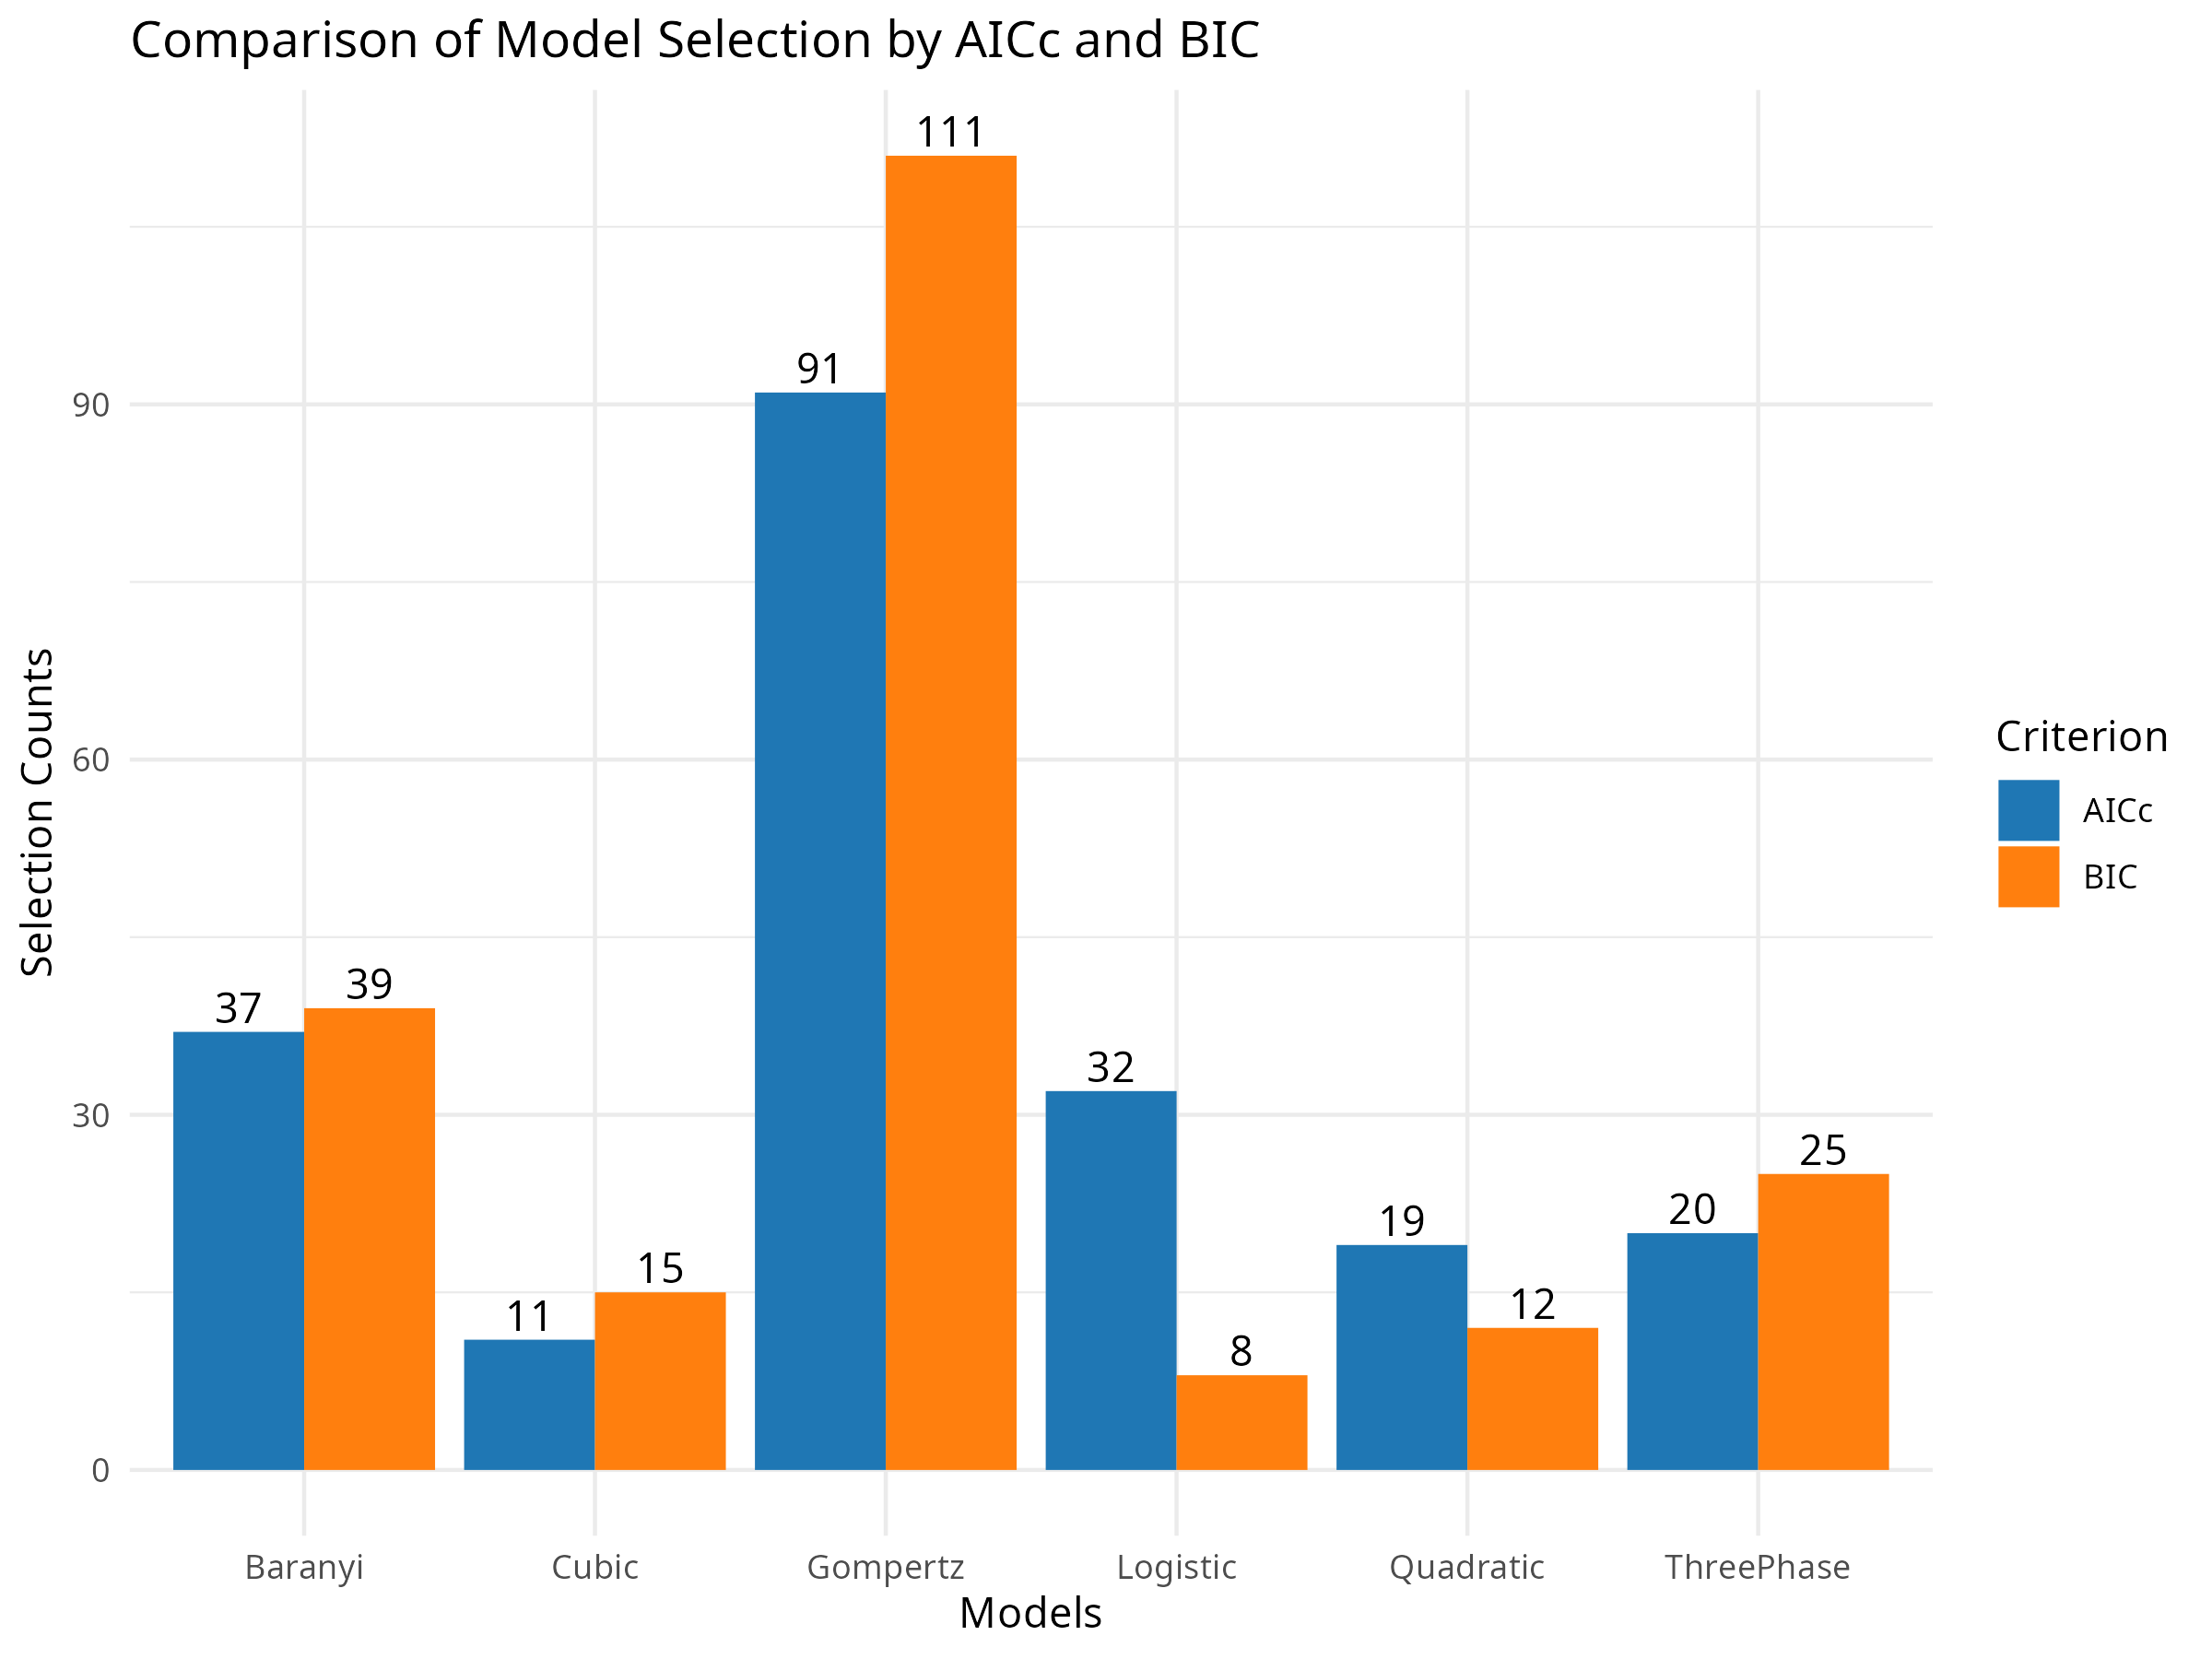
\includegraphics[width=0.7\textwidth]{"../results/model_selection_comparison.png"}
    \caption{Comparison of Model Selection Based on AICc and BIC. This bar chart presents the number of times each model was selected as the best according to Akaike Information Criterion corrected for small sample sizes (AICc) and Bayesian Information Criterion (BIC). The two colors represent the different selection criteria, with AICc and BIC often favoring different models.}
    \label{fig:model_selection}
\end{figure}

\vspace{-1em} % Reduce vertical space between figures (adjust as needed)

\begin{figure}[H]
    \centering
    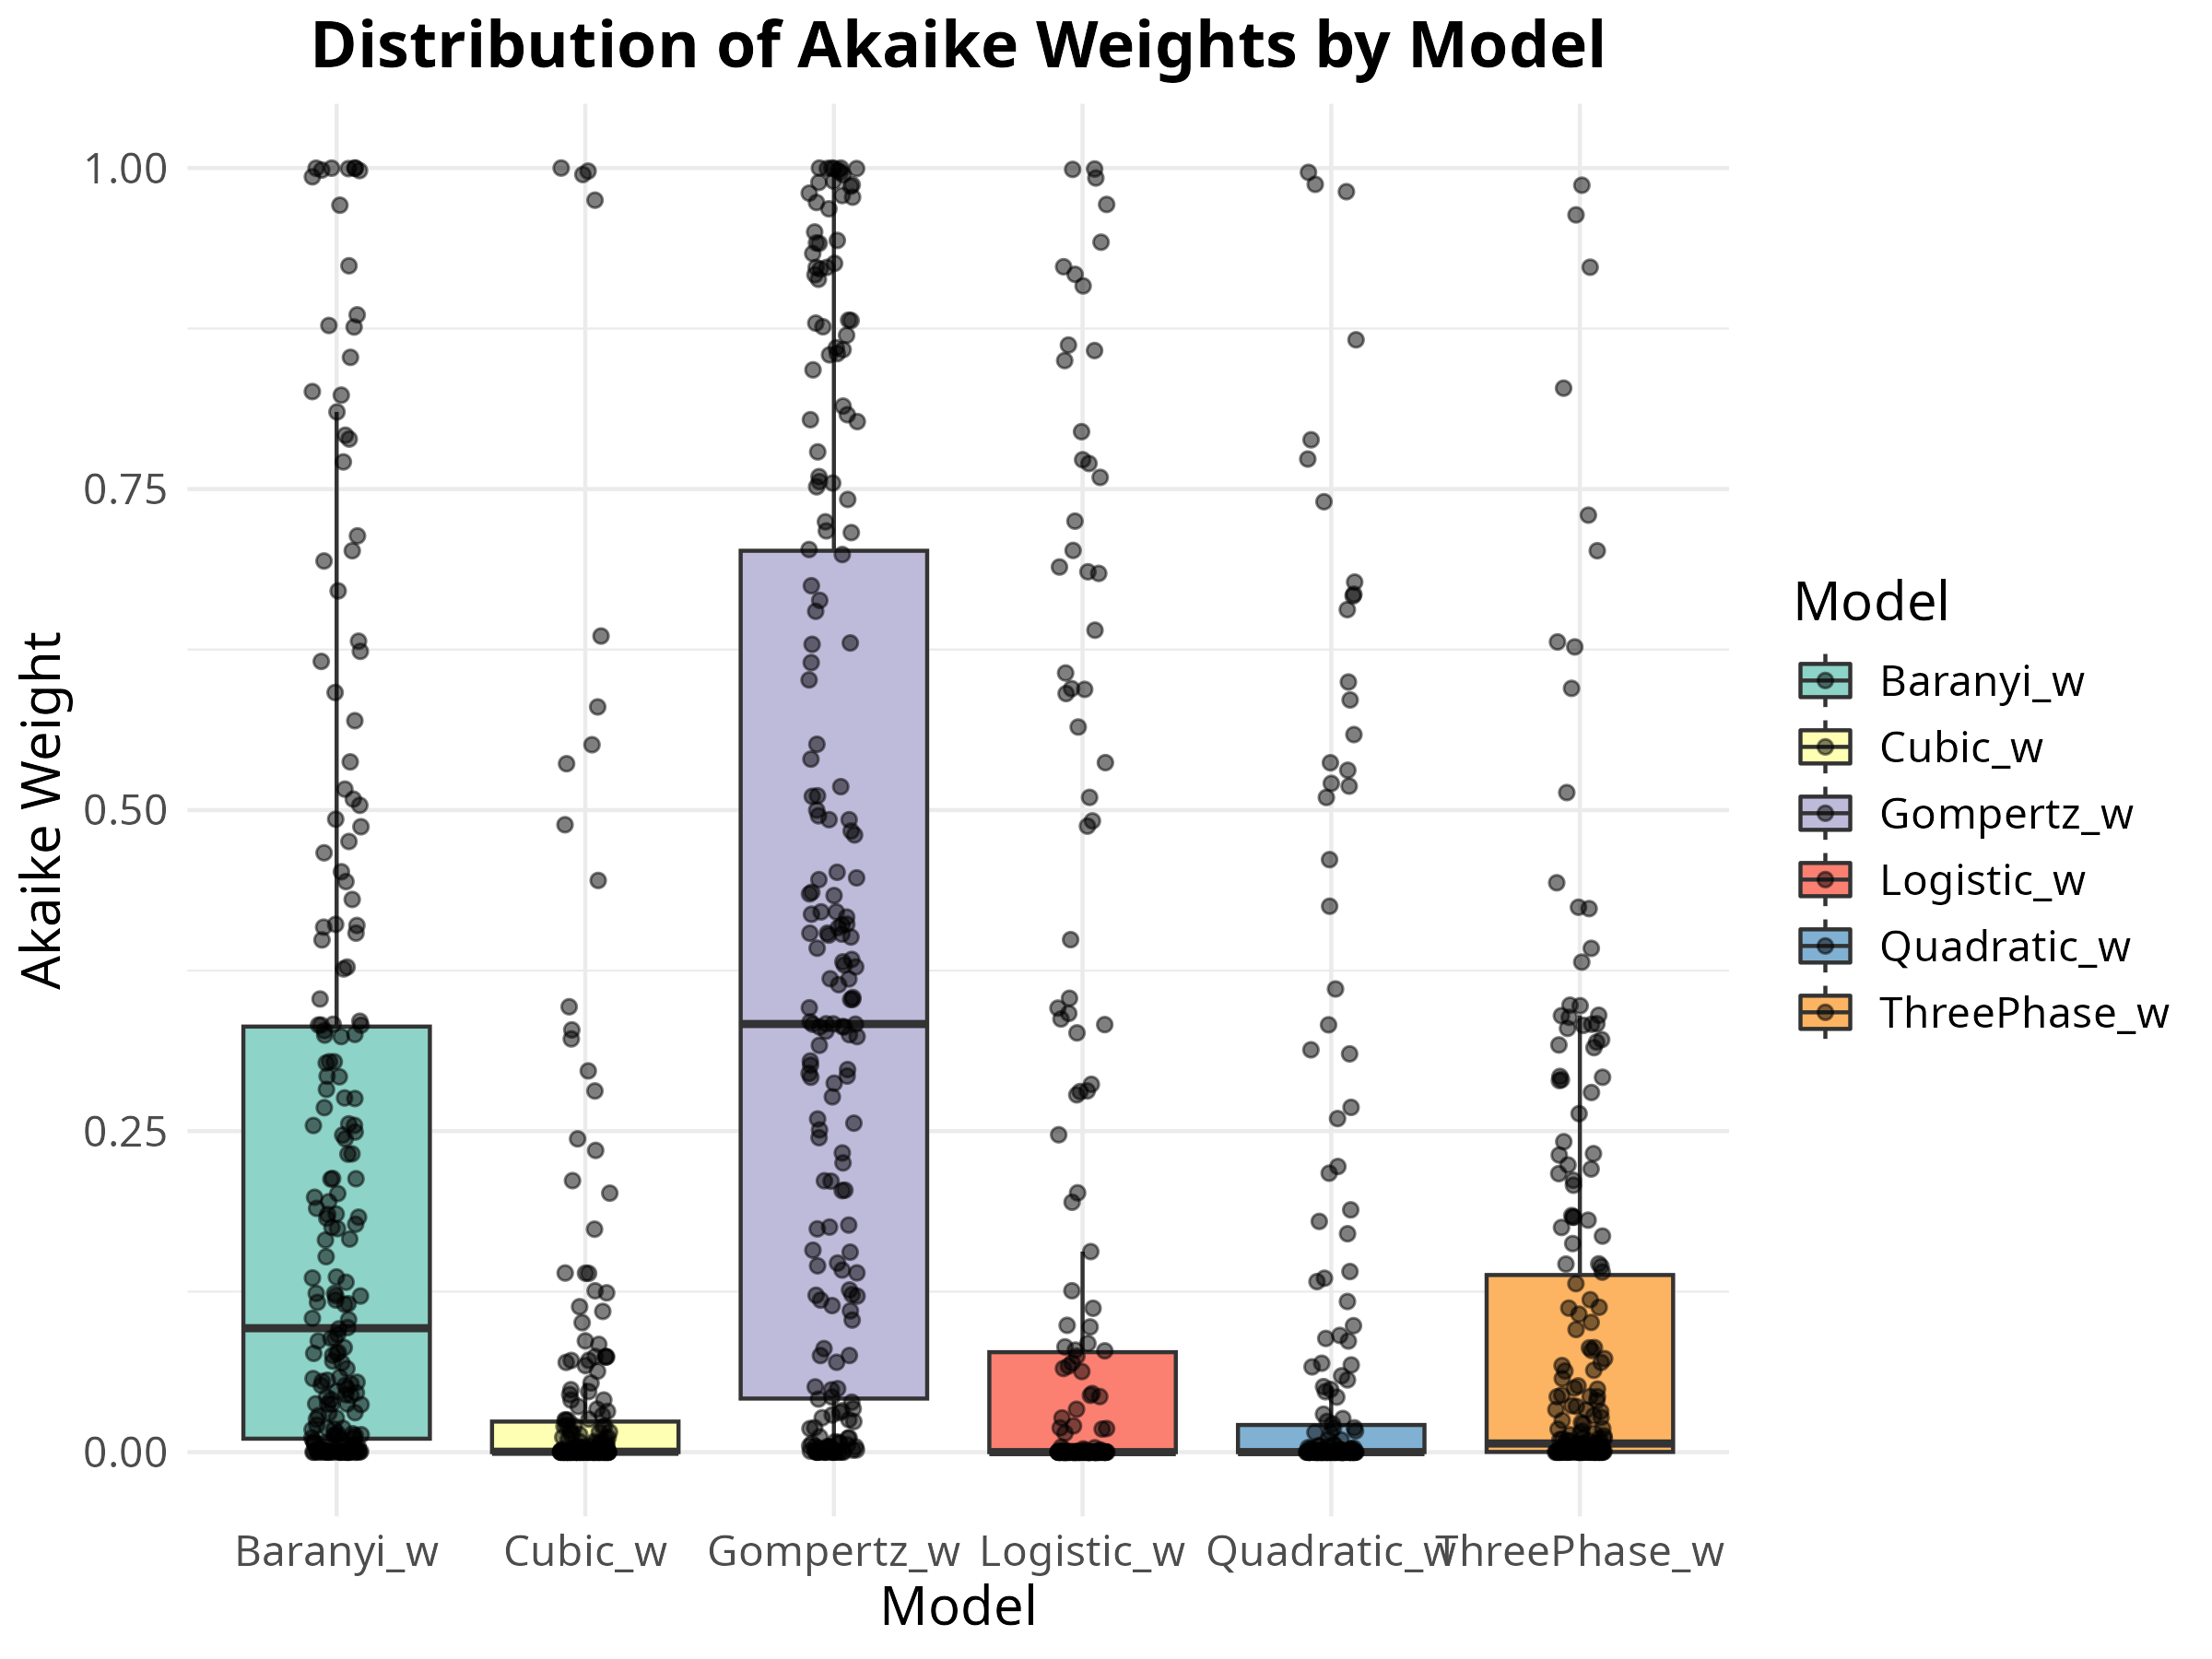
\includegraphics[width=0.7\textwidth]{../results/akaike_weights_boxplot_nice.png}
    \caption{Distribution of Akaike Weights Across Models. This boxplot illustrates the Akaike weight distributions for six models: Baranyi, Cubic, Gompertz, Logistic, Quadratic, and Three-Phase. The Akaike weight represents the relative likelihood of each model being the best fit. Models with higher median Akaike weights are more frequently selected as the best. Some models show consistently low Akaike weights, indicating weaker performance. Individual points represent data variability, with black dots showing Akaike weights for each model.}
    \label{fig:akaike_weights}
\end{figure}

\begin{table}[htbp]
\centering
\caption{Number of Fitting Failures for Each Model}
\label{tab:fitting_failures}
\begin{tabular}{l c}
\hline
Model & Count \\
\hline
Quadratic & 0 \\
Cubic     & 0 \\
Logistic  & 96 \\
Gompertz  & 9 \\
Baranyi   & 9 \\
ThreePhase& 1 \\
\hline
\end{tabular}
\end{table}

\section{Discussion}
Although the improved Gompertz model outperformed other models in terms of the frequency of being selected as the best-fitting model and its AICc weight (0.39), this weight does not indicate an absolute advantage. Since an AICc weight closer to 1 represents a higher probability of being the optimal model \citep{JohnsonOmland2004}, a value of 0.39 suggests that model selection should still consider multiple factors rather than relying solely on this single criterion. Therefore, although the improved Gompertz model performs well, it should not be regarded as the only optimal model and requires further evaluation.

In terms of linear models, although quadratic and cubic polynomial models often achieve stable numerical convergence, they are typically purely mathematical models and thus lack biological significance. These models fail to accurately depict the plateau phase in microbial growth curves, and in my fitted dataset, they sometimes predict a decline in growth trends over longer time scales, which contradicts the actual microbial growth process(Figure 3). The three-phase linear model (piecewise linear model) captures nonlinear transitions by dividing the growth curve into the lag phase, exponential growth phase, and stationary phase. However, when the phase transitions in actual growth data are smoother, or when the data itself does not exhibit a distinct three-phase structure (Figure 4), the abrupt breakpoints in this model may lead to poor local fit, resulting in biological inconsistencies in certain datasets.

\begin{figure}[htbp]
  \centering

  %----- Left Figure (Figure 3) -----
  \begin{minipage}[t]{0.48\textwidth}
    \centering
    \includegraphics[width=\linewidth]{6models_ID_11.png}
    \captionof{figure}{%
      Fitted results for dataset \textbf{ID = 11} . 
      The Quadratic and Cubic polynomial models often achieve stable numerical convergence 
      but lack biological significance. They fail to accurately depict the plateau phase 
      and may even predict a decline in growth trends over longer time scales, 
      which contradicts actual microbial growth.
    }
    \label{fig:ID11}
  \end{minipage}
  \hfill
  %----- Right Figure (Figure 4) -----
  \begin{minipage}[t]{0.48\textwidth}
    \centering
    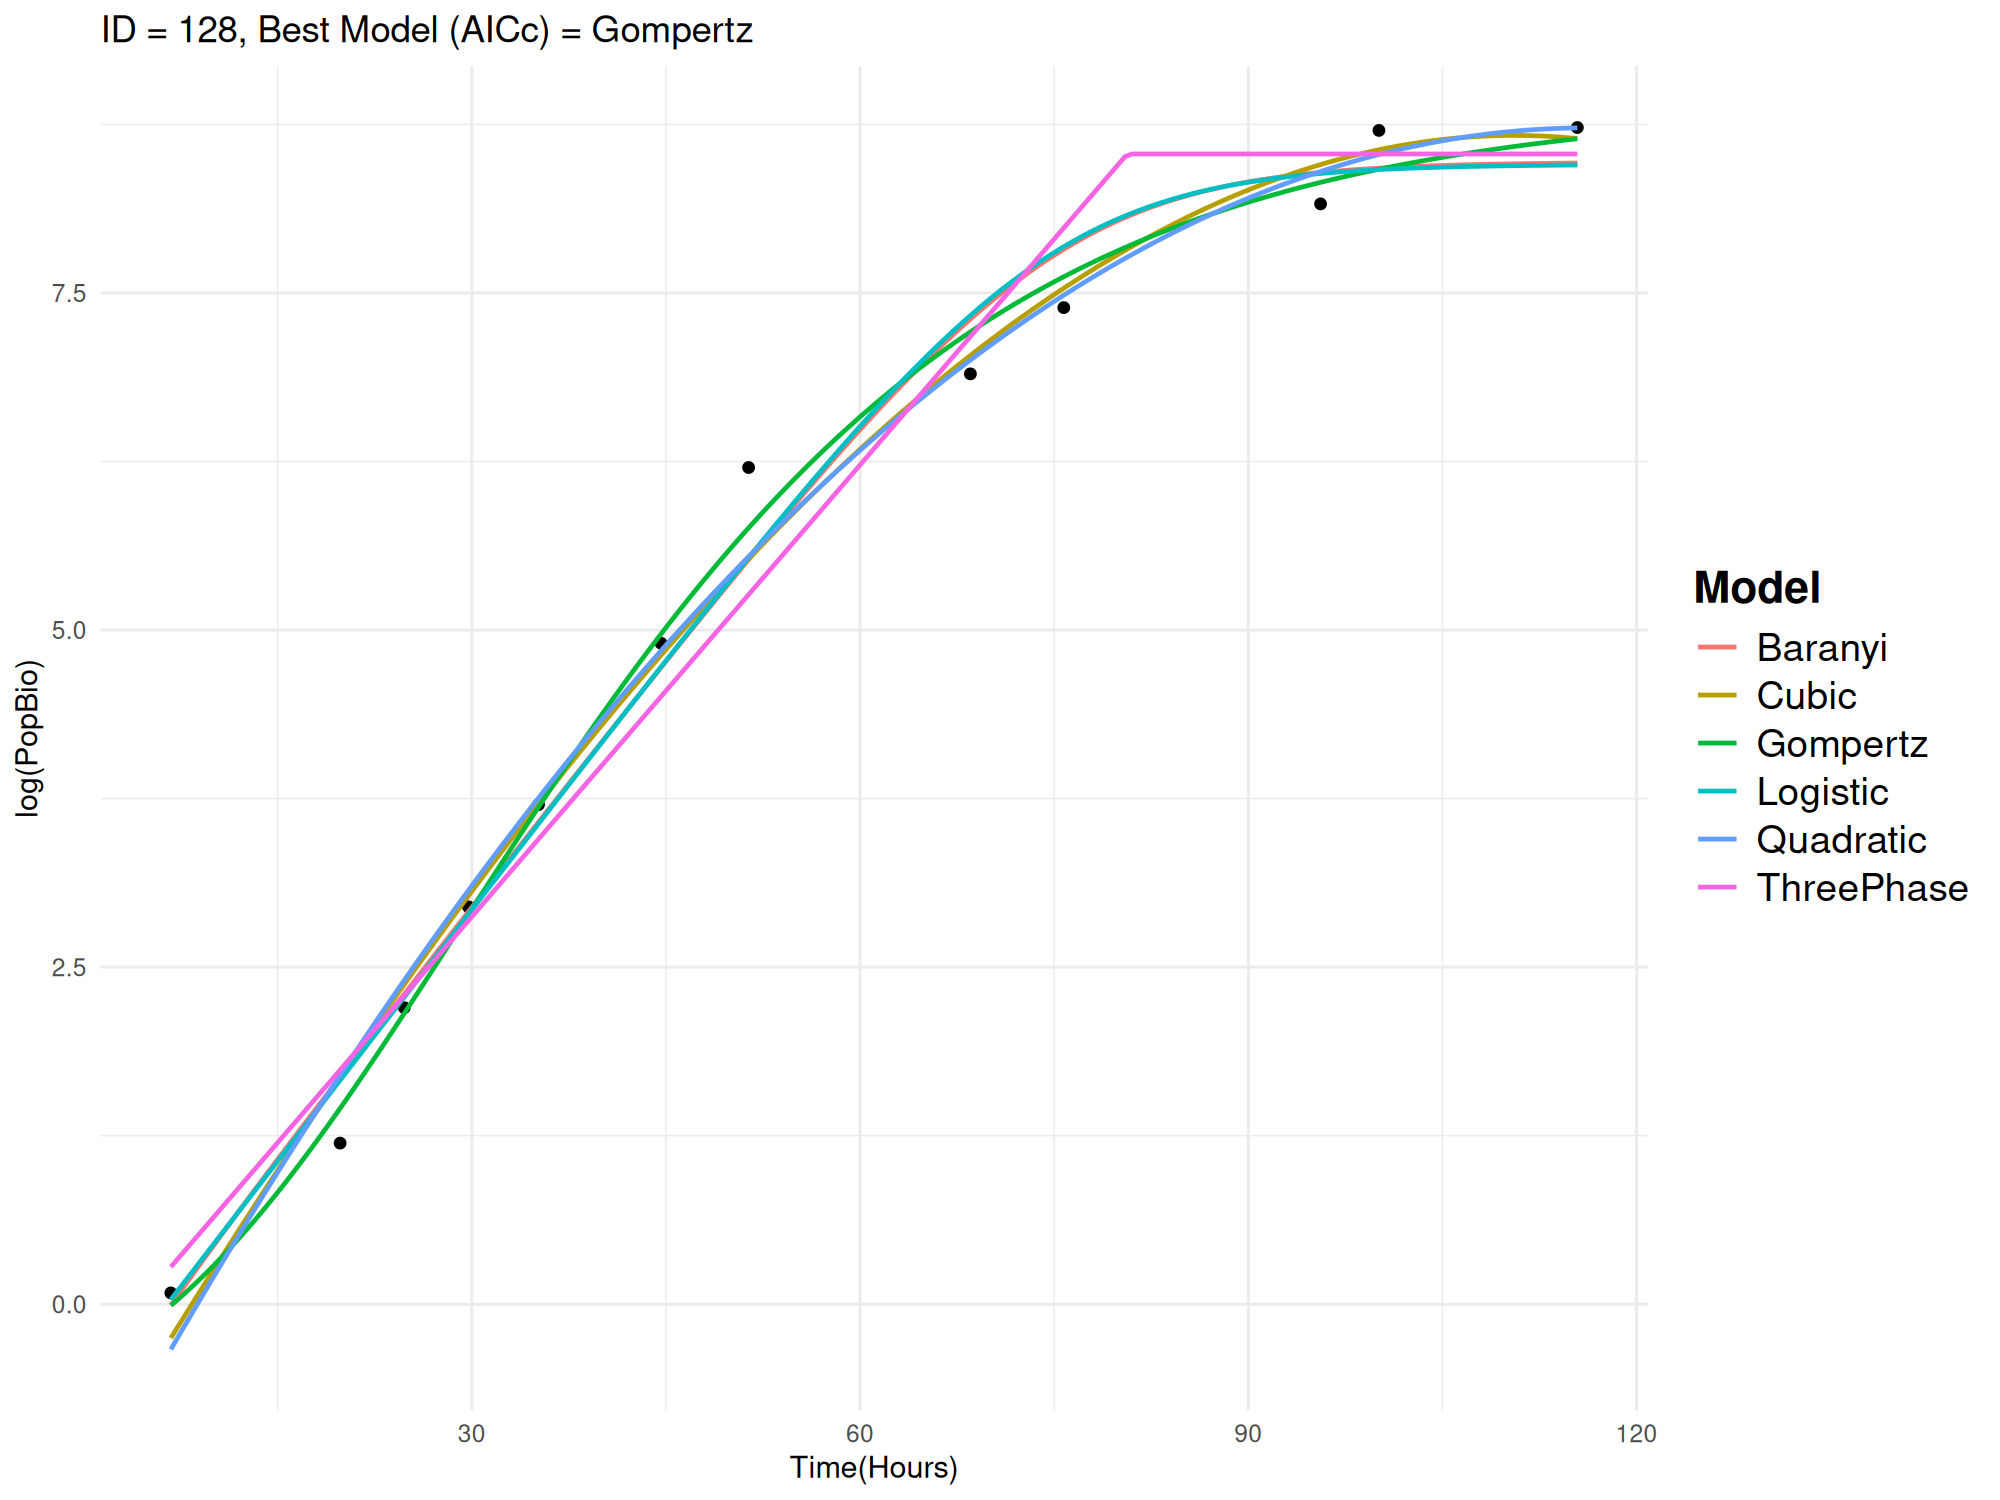
\includegraphics[width=\linewidth]{6models_ID_128.png}
    \captionof{figure}{%
      Fitted results for dataset \textbf{ID = 128} .
      The Three-Phase Linear Model (piecewise linear) captures nonlinear transitions 
      by splitting the growth curve into distinct phases (lag, exponential, and stationary). 
      However, when actual growth data are smoother or do not exhibit a clear three-phase 
      structure, its abrupt breakpoints can produce poor local fits and lead to biological 
      inconsistencies.
    }
    \label{fig:ID128}
  \end{minipage}

\end{figure}

In nonlinear S-shaped growth models, the Logistic, Baranyi, and improved Gompertz models each have their advantages and limitations. The Logistic model exhibited the worst convergence, failing to converge in 96 out of 210 datasets. This may be related to its core assumption that the growth curve follows a symmetric S-shape, implying that the durations of the lag phase and the exponential growth phase are similar \citep{LoGrasso2023}. However, in actual experiments, microbial growth curves are often asymmetric. Moreover, in the dataset used in this study, many experiments did not fully cover the entire microbial growth process. When the available data only capture part of the growth stages, it becomes challenging to accurately estimate the environmental carrying capacity ($K$), leading to fitting failures or instability. For instance, in the ID = 67 dataset(Figure 5), the exponential growth phase exhibits significant asymmetry, and the lag phase is absent, which may explain the convergence failure of the Logistic model. Additionally, the Logistic model systematically overestimated the initial population size ($N_0$), as observed in the box plot (Figure 6), where a large number of data points appeared as extreme upper-bound outliers. This may be due to an extended actual lag phase, causing the model to artificially increase $N_0$ to match the growth curve, or the lack of early (low biomass) observations in the data, leading the Logistic model to misinterpret the growth start time and consequently overestimate $N_0$. Although this study used AICc and other data comparisons for model evaluation, the experimental results align closely with the findings of \citet{Zwietering1990}, who compared models using t-tests and F-tests. Their study also indicated that the Logistic model has a narrower applicability and is unsuitable for most experimental data, whereas the Gompertz model is relatively more appropriate.
\begin{figure}[htbp]
  \centering
%--- Left Figure (Figure 5) ---
  \begin{minipage}[t]{0.45\textwidth}
    \centering
    % Assume the image filename is ID67.png
    \includegraphics[width=\linewidth]{6models_ID_67.png}
    \captionof{figure}{%
      \textbf Fitted results for dataset ID=67. 
      The exponential growth phase exhibits significant asymmetry, 
      and the lag phase is absent, which may explain the convergence failure 
      of the Logistic model. Because the model failed to converge, 
      no fitted line is shown for the Logistic model.
    }
    \label{fig:ID67}
  \end{minipage}
  \hfill
  %--- Right Figure (Figure 6) ---
  \begin{minipage}[t]{0.45\textwidth}
    \centering
    % Assume the image filename is param_N0.png
    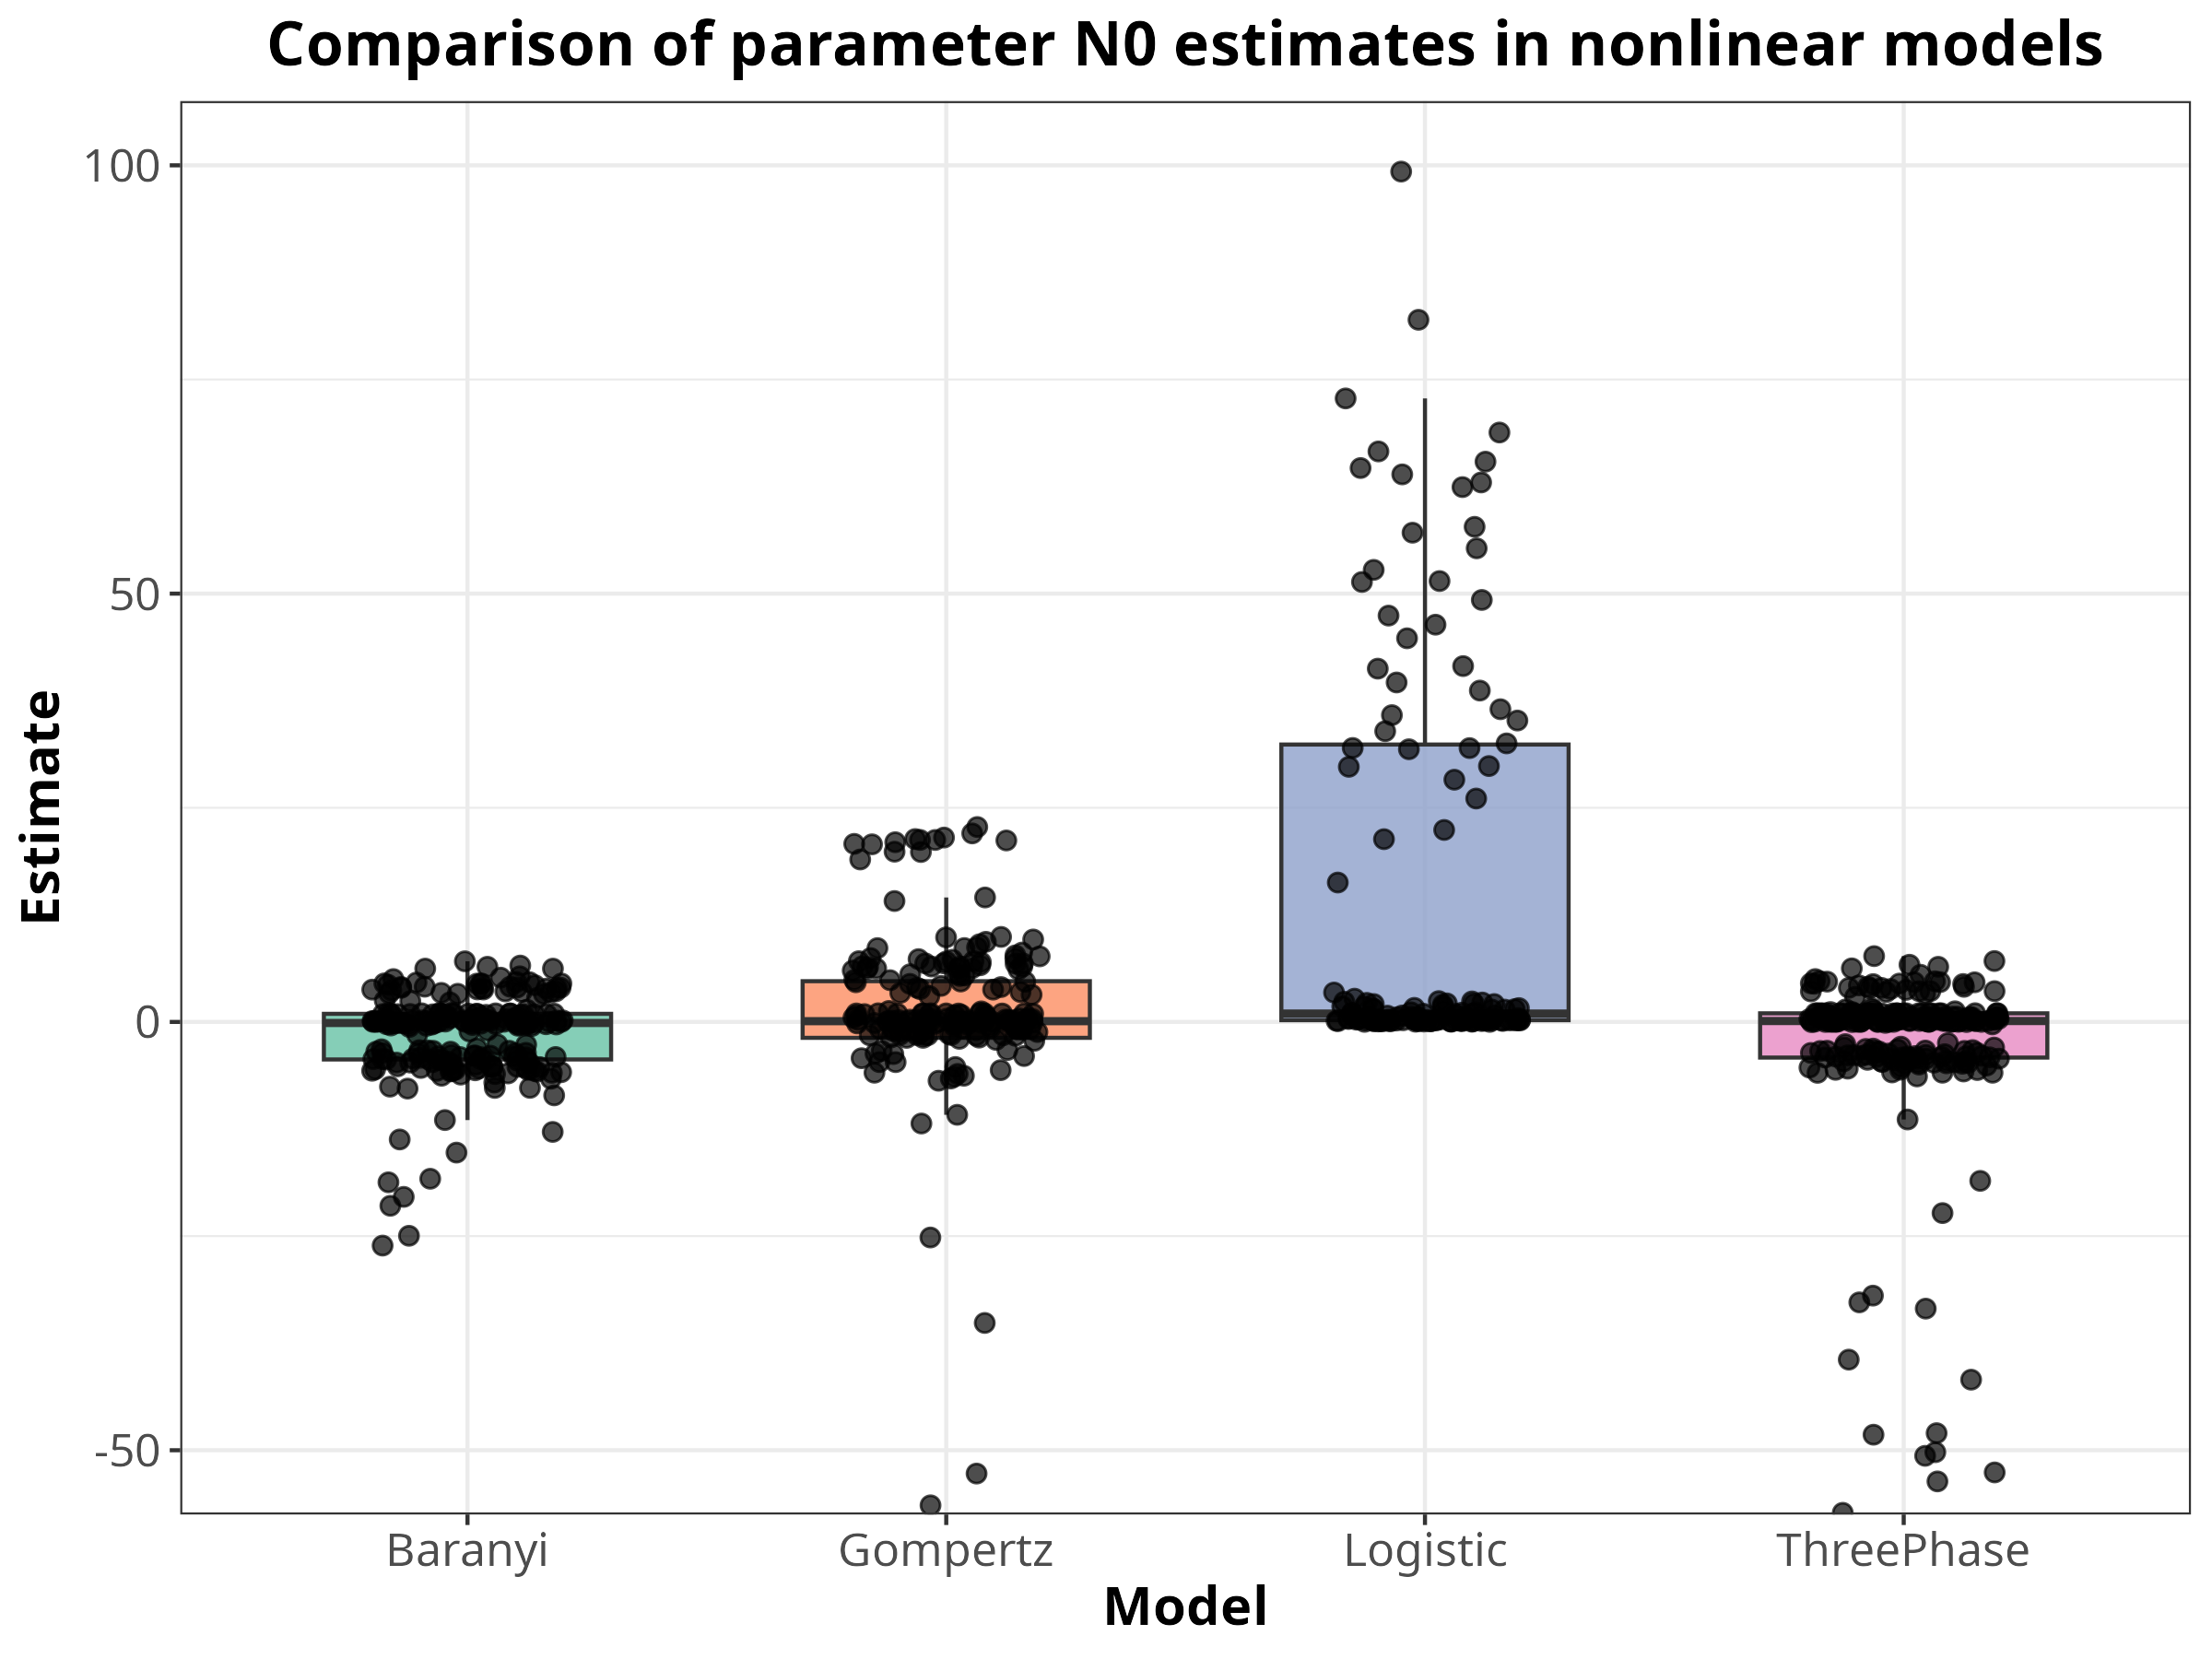
\includegraphics[width=\linewidth]{nonlinear_parameter_comparison_N0.png}
    \captionof{figure}{%
      \textbf Comparison of \(N_0\) parameter estimates 
      across different nonlinear models. 
      This boxplot displays the distribution of \(N_0\) estimates for each model, 
      with black dots indicating individual fits. 
      Models with higher or more variable estimates may reflect 
      greater uncertainty or sensitivity in parameter estimation.
    }
    \label{fig:paramN0}
  \end{minipage}

\end{figure}
Although the Baranyi model theoretically incorporates a well-defined biological framework for modeling the lag phase and is generally capable of reasonably estimating key parameters (such as lag phase duration and maximum growth rate), its support rate in this study was lower than expected. The primary reason for this may be that the Baranyi model relies on a ``physiological state variable'' to describe the dynamic changes of the lag phase. However, if the dataset lacks sufficient observations during the lag phase, the parameter $h_0$ cannot be accurately estimated, thereby affecting the entire fitting process. This limitation highlights that even theoretically sound models may underperform compared to more flexible empirical models when critical data points are missing.

Since the improved Gompertz model is more flexible than the Logistic model and can represent asymmetric S-shapes \citep{Gibson1987}, it generally performs well. However, its flexibility should be considered dialectically. Models with higher degrees of parameter freedom can usually better fit complex growth curves, but they are also more susceptible to noise and may even lead to overfitting \citep{Merow2014}. In some Gompertz model fittings in this study, the standard errors of parameter estimates were relatively high, which may be a reflection of this issue. I found that the improved Gompertz model overestimated $r_{\text{max}}$ compared to other models (Figure7), possibly due to its fitting approach during the exponential growth phase, which amplifies the steep portion of the growth curve. This trend is consistent with the findings of \citet{Membre2002}, who observed that the Gompertz equation systematically overestimated $r_{\text{max}}$ in the modeling of \textit{Listeria monocytogenes} growth. Therefore, in practical applications, it is necessary to balance the biological interpretability of parameters with the need to avoid model overfitting, ensuring that the model is not merely capturing random fluctuations in the data \citep{CawleyTalbot2010}, but truly reflecting the underlying biological processes.

\begin{figure}[htbp]
    \centering
    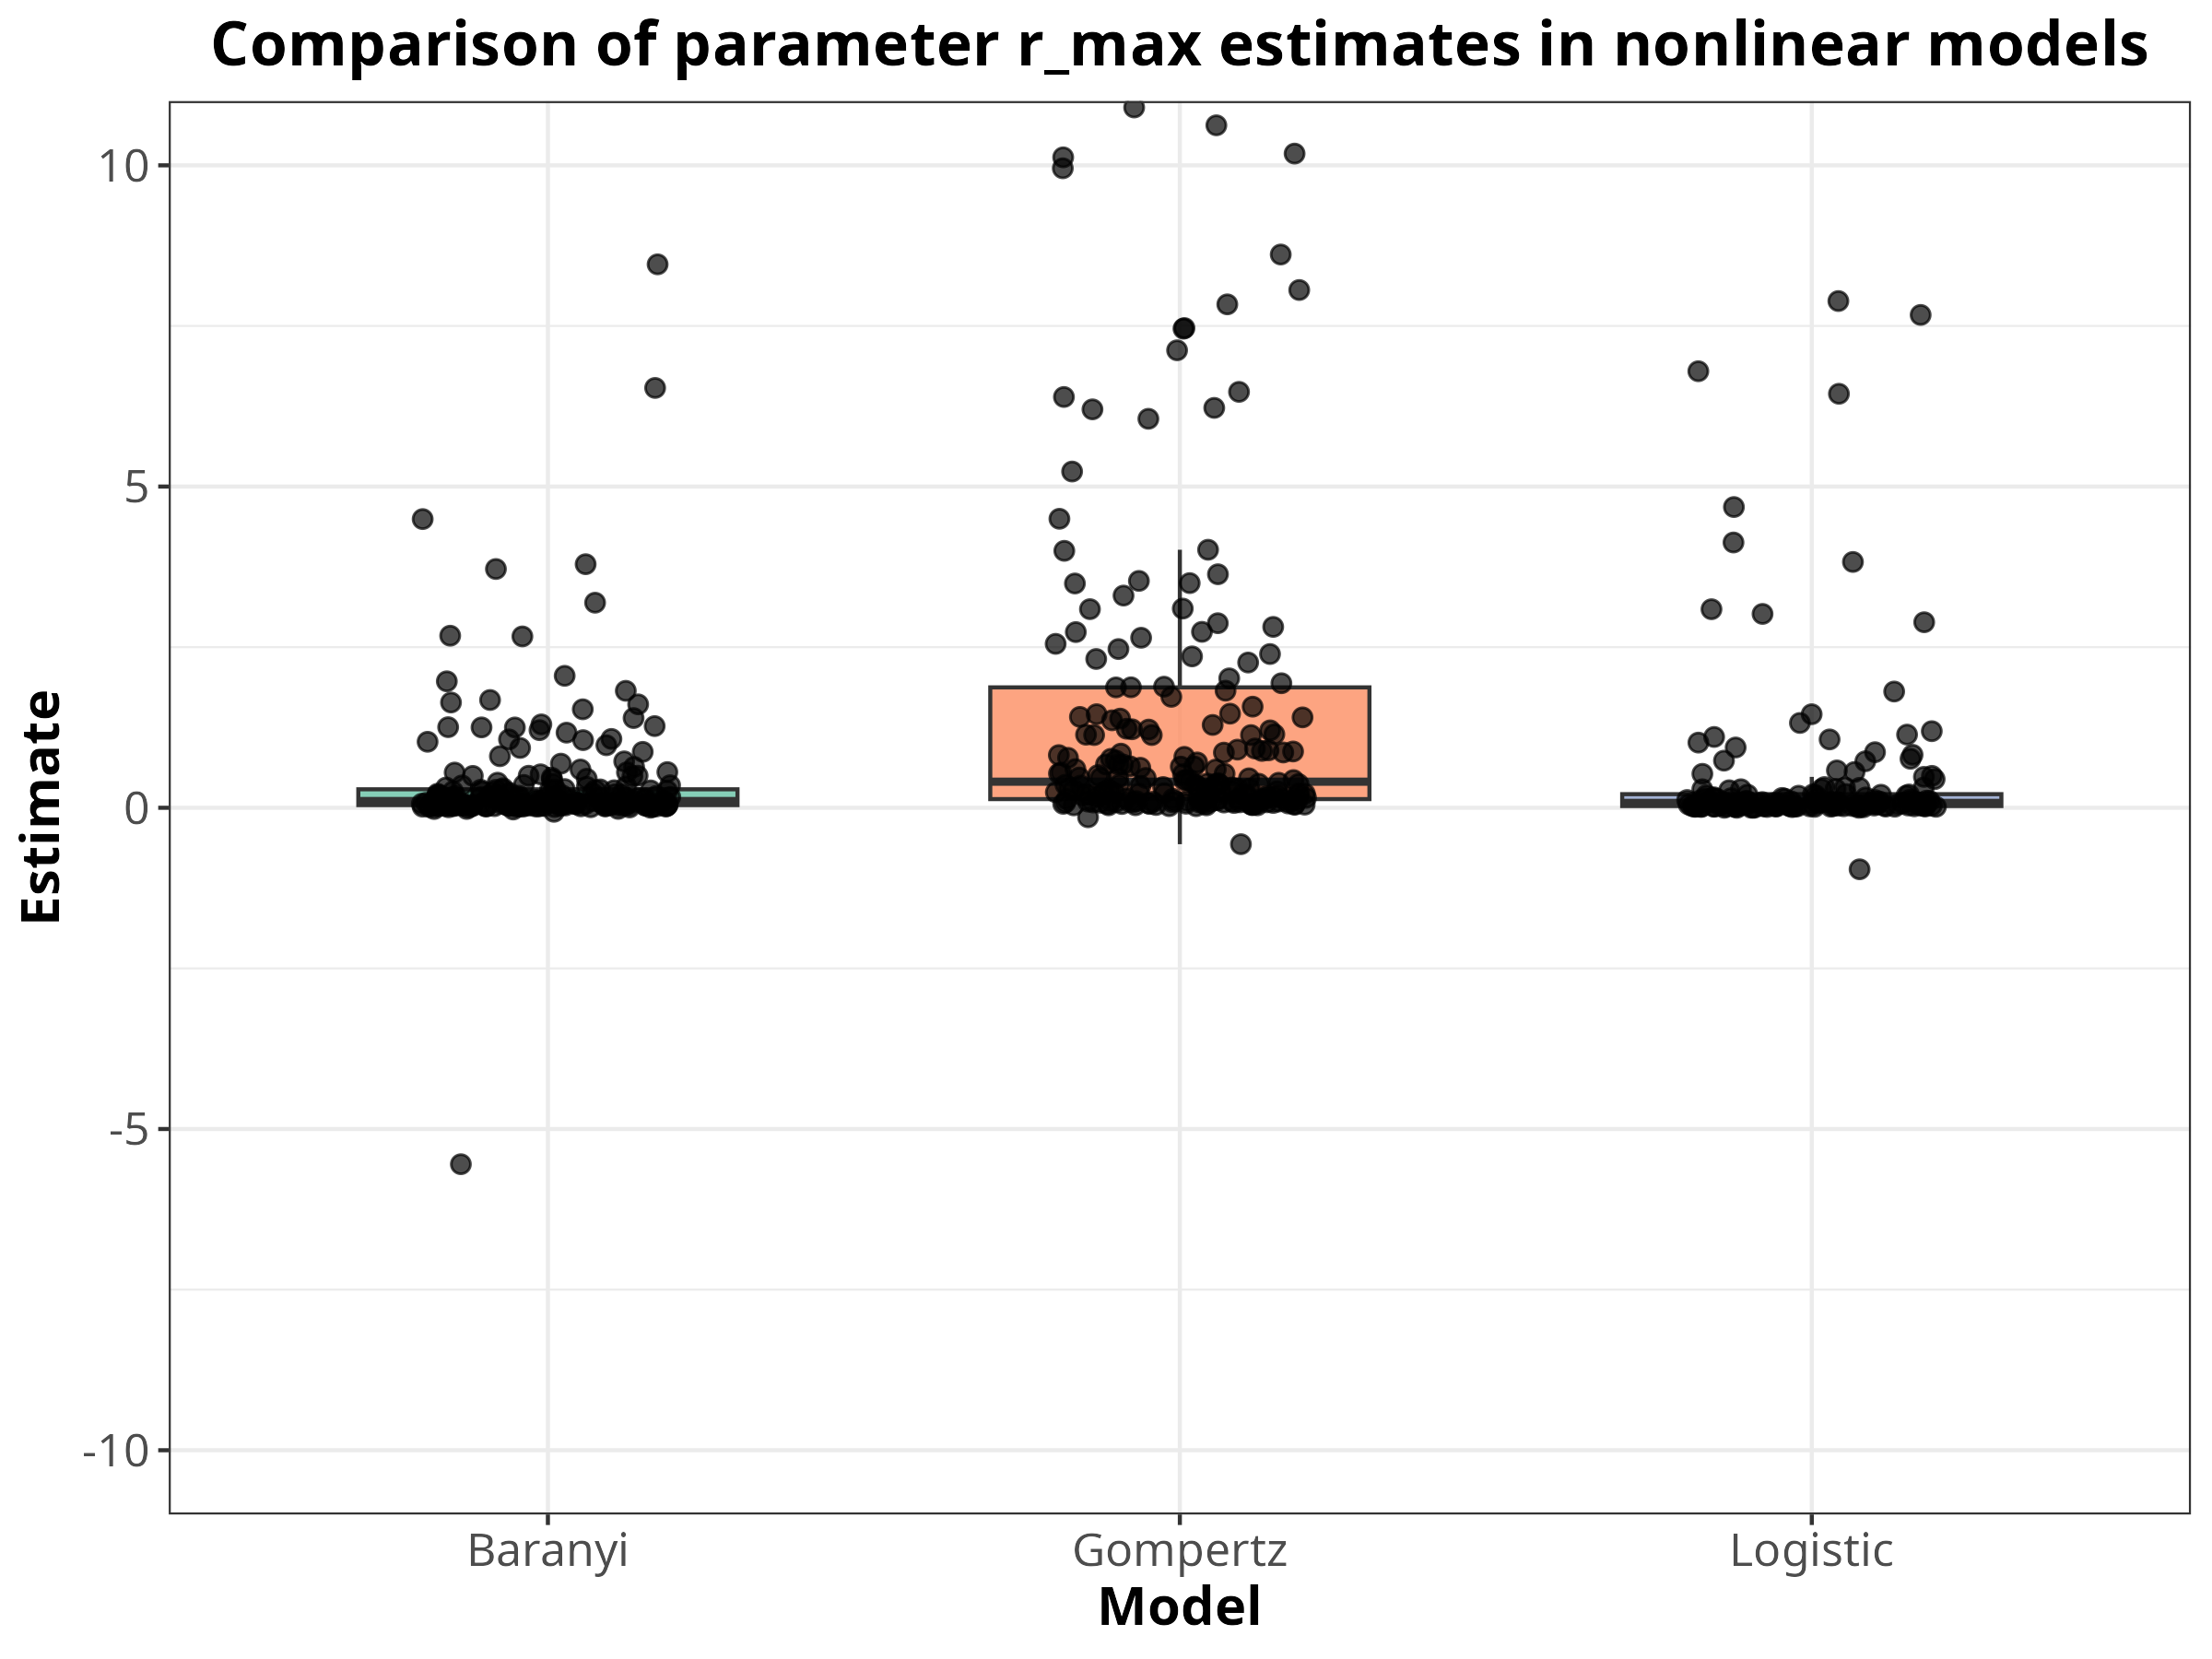
\includegraphics[width=0.8\textwidth]{nonlinear_parameter_comparison_r_max.png}
    \caption{%
        \textbf Comparison of parameter \(r_{\max}\) estimates in nonlinear models.
        The boxplot shows the distribution of \(r_{\max}\) (maximum growth rate) for each model. 
    }
    \label{fig:r_max_estimates}
\end{figure}

\begin{figure}[htbp]
    \centering
    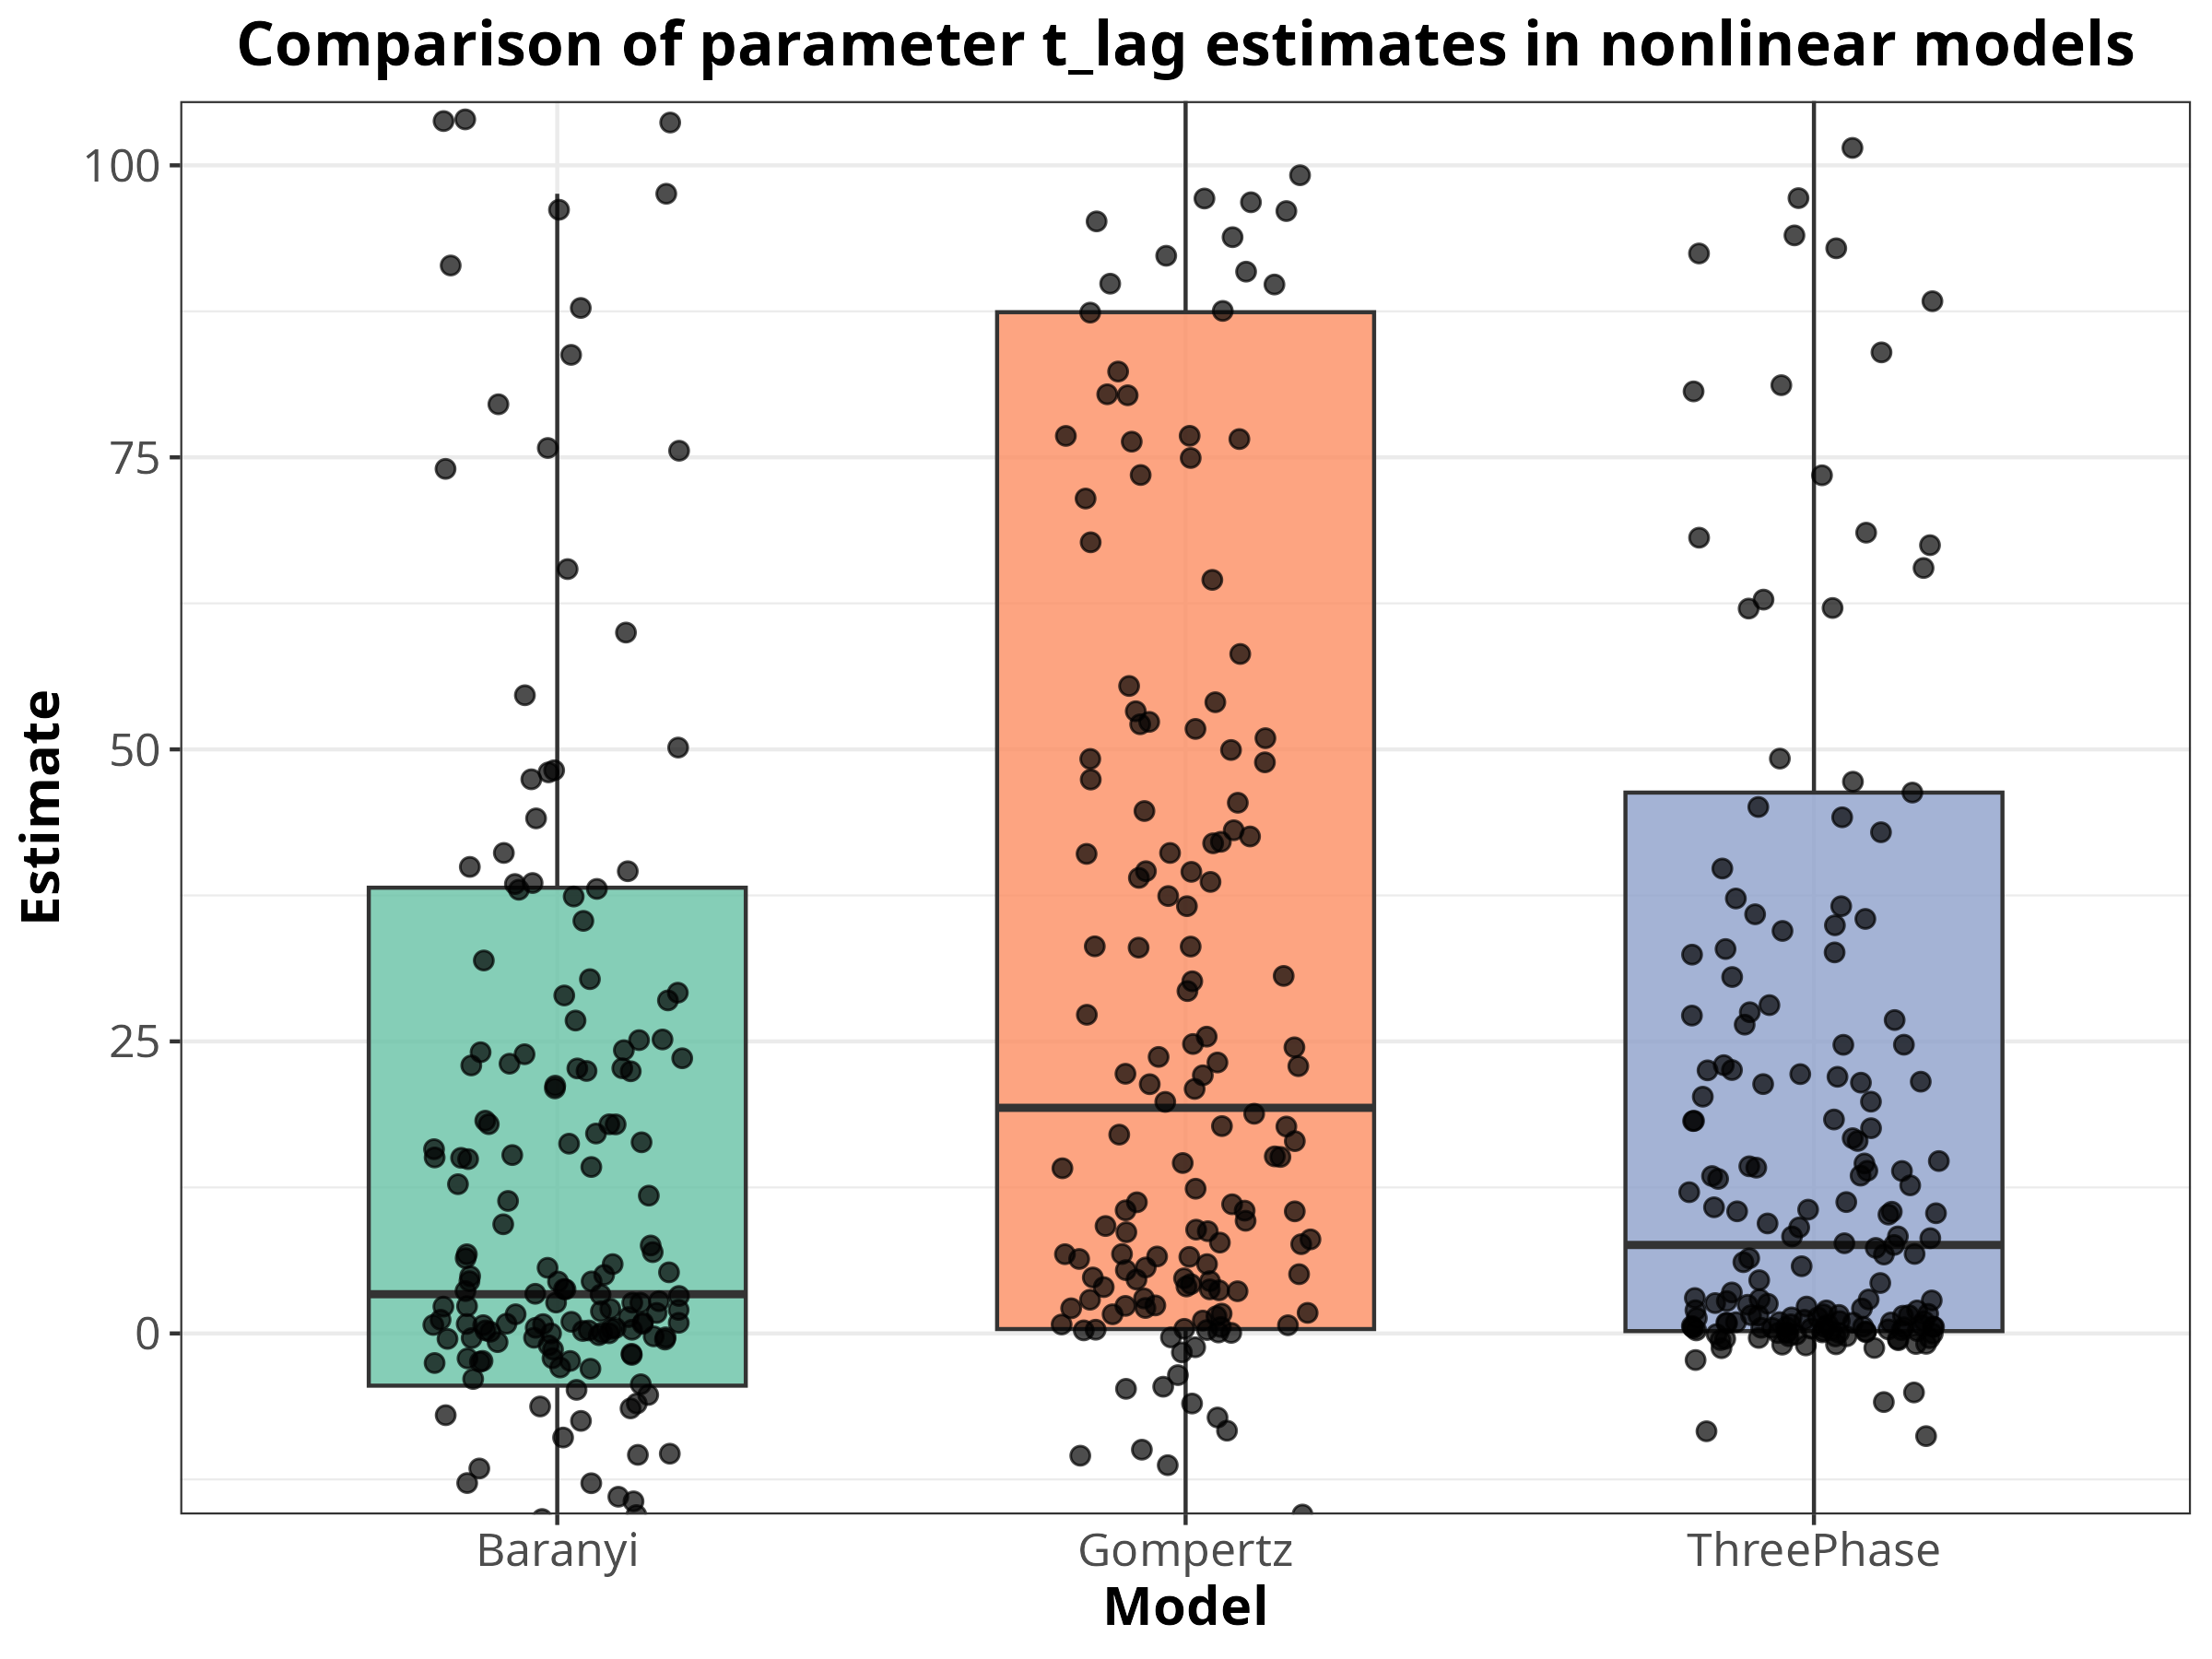
\includegraphics[width=0.8\textwidth]{nonlinear_parameter_comparison_t_lag.png}
    \caption{%
        \textbf Comparison of parameter \(t_{\mathrm{lag}}\) estimates in nonlinear models
        (Baranyi, Gompertz, and Three-Phase). The boxplot displays the range and distribution of
        \(t_{\mathrm{lag}}\) values for each model.
    }
    \label{fig:t_lag_estimates}
\end{figure}
In microbial growth modeling, a key challenge is balancing biological realism with the inherent mathematical assumptions of the models. Even complex mechanistic models often assume that the lag phase can be represented by a single parameter or a physiological state variable. However, in reality, the lag phase is influenced by multiple factors, such as inoculation history, cell-to-cell variability, and adaptive stress responses, which may not be fully captured by a single-state parameter \citep{BaranyiRoberts1994}. Therefore, if experimental data do not adequately cover the early adaptation phase, overestimation or underestimation of the lag phase can impact the overall fitting performance, ultimately weakening the theoretical advantages of models that explicitly incorporate lag phase parameters. This contradiction between the mathematical elegance of these models and the complexity of real-world data explains why no single model consistently performs best under all conditions.

Another layer of complexity arises from the fact that many experimental datasets are incomplete, covering only certain portions of the growth curve. If researchers collect biomass measurements at fewer time points or fail to capture the early or late growth phases, even well-designed models may struggle to estimate parameters reliably. For example, if data do not sufficiently cover the stationary phase, Logistic and Baranyi models may introduce significant biases when estimating the environmental carrying capacity ($K$). Conversely, if lag phase data are missing, all models that assume the presence of a lag phase (such as Baranyi and Gompertz) may inaccurately estimate $t_{\text{lag}}$, affecting the final fitting results. Additionally, traditional nonlinear least squares (NLS) or maximum likelihood estimation (MLE) methods may become trapped in local minima if initial parameter selection is suboptimal, thereby impacting model convergence \citep{BurnhamAnderson2002}. These issues highlight the need for carefully designed data collection strategies to ensure comprehensive coverage of all critical growth phases, such as implementing more frequent automated sampling or conducting preliminary studies before formal experiments to determine reasonable ranges for the lag and stationary phases.

In conclusion, the findings of this study indicate that no single model is optimal across all datasets. Data quality and completeness are crucial for the reliable estimation of key parameters. Even theoretically more biologically mechanistic models, such as the Baranyi model, may perform poorly if lag phase data are insufficient. Similarly, highly flexible models, such as the improved Gompertz model, can adapt to various datasets but may introduce parameter uncertainty when data are sparse or noisy. Therefore, future research should integrate more comprehensive data collection, robust parameter estimation methods, and transparent model comparison strategies to enhance the reliability and biological applicability of microbial growth predictions.
\clearpage
\bibliographystyle{apalike} 
\bibliography{references}   


\end{document}

